%definira klasu dokumenta 
\documentclass[12pt]{report} 

%prostor izmedu naredbi \documentclass i \begin{document} se zove uvod. U njemu se nalaze naredbe koje se odnose na cijeli dokument

%osnovni LaTex ne može riješiti sve probleme, pa se koriste različiti paketi koji olakšavaju izradu željenog dokumenta
\usepackage[croatian]{babel} 
\usepackage{amssymb}
\usepackage{amsmath}
\usepackage{txfonts}
\usepackage{mathdots}
\usepackage{titlesec}
\usepackage{array}
\usepackage{lastpage}
\usepackage{etoolbox}
\usepackage{longtable, tabu}
\usepackage{color, colortbl}
\usepackage{adjustbox}
\usepackage{geometry}
\usepackage[classicReIm]{kpfonts}
\usepackage{hyperref}
\usepackage{fancyhdr}

\usepackage{float}
\usepackage{setspace}
\restylefloat{table}


\patchcmd{\chapter}{\thispagestyle{plain}}{\thispagestyle{fancy}}{}{} %redefiniranje stila stranice u paketu fancyhdr

%oblik naslova poglavlja
\titleformat{\chapter}{\normalfont\huge\bfseries}{\thechapter.}{20pt}{\Huge}
\titlespacing{\chapter}{0pt}{0pt}{40pt}


\linespread{1.3} %razmak između redaka

\geometry{a4paper, left=1in, top=1in,}  %oblik stranice

\hypersetup{ colorlinks, citecolor=black, filecolor=black, linkcolor=black,	urlcolor=black }   %izgled poveznice


%prored smanjen između redaka u nabrajanjima i popisima
\newenvironment{packed_enum}{
	\begin{enumerate}
		\setlength{\itemsep}{0pt}
		\setlength{\parskip}{0pt}
		\setlength{\parsep}{0pt}
	}{

\end{enumerate}}

\newenvironment{packed_item}{
	\begin{itemize}
		\setlength{\itemsep}{0pt}
		\setlength{\parskip}{0pt}
		\setlength{\parsep}{0pt}
	}{\end{itemize}}


%boja za privatni i udaljeni kljuc u tablicama
\definecolor{LightBlue}{rgb}{0.9,0.9,1}
\definecolor{LightGreen}{rgb}{0.9,1,0.9}


%podesavanje zaglavlja i podnožja

\pagestyle{fancy}
\lhead{Programsko inženjerstvo}
\rhead{Projektni zadatak}
\lfoot{springRolice}
\cfoot{stranica \thepage/\pageref{LastPage}}
\rfoot{\today}
\renewcommand{\headrulewidth}{0.2pt}
\renewcommand{\footrulewidth}{0.2pt}


\begin{document} 
	
	
	
	\begin{titlepage}
		\begin{center}
			\vspace*{\stretch{1.0}} %u kombinaciji s ostalim \vspace naredbama definira razmak između redaka teksta
			\LARGE Programsko inženjerstvo\\
			\large Ak. god. 2020./2021.\\
			
			\vspace*{\stretch{3.0}}
			
			\huge Zamjena soba\\
			\Large Dokumentacija, Rev. \textit{1}\\
			
			\vspace*{\stretch{12.0}}
			\normalsize
			Grupa: \textit{springRolice}\\
			Voditelj: \textit{Mateja Iveta}\\
			
			
			\vspace*{\stretch{1.0}}
			Datum predaje: \textit{$<$dan$>$. $<$mjesec$>$. $<$godina$>$.}\\
			
			\vspace*{\stretch{4.0}}
			
			Nastavnik: \textit{Ivana Cepetić}\\
			
		\end{center}
		
		
	\end{titlepage}
	
	
	\tableofcontents
	
	\chapter{Dnevnik promjena dokumentacije}
		
		\textbf{\textit{Kontinuirano osvježavanje}}\\
				
		
		\begin{longtabu} to \textwidth {|X[2, l]|X[13, l]|X[3, l]|X[3, l]|}
			\hline \multicolumn{1}{|l|}{\textbf{Rev.}}	& \multicolumn{1}{l|}{\textbf{Opis promjene/dodatka}} & \multicolumn{1}{|l|}{\textbf{Autori}} & \multicolumn{1}{l|}{\textbf{Datum}} \\[3pt] \hline
			\endfirsthead
			
			\hline \multicolumn{1}{|l|}{\textbf{Rev.}}	& \multicolumn{1}{l|}{\textbf{Opis promjene/dodatka}} & \multicolumn{1}{|l|}{\textbf{Autori}} & \multicolumn{1}{l|}{\textbf{Datum}} \\[3pt] \hline
			\endhead
			
			\hline 
			\endlastfoot
			
			0.1 & Napravljen predložak.	& Ivošević & 22.08.2013. 		\\[3pt] \hline 
			0.2	& Dopisane upute za povijest dokumentacije.\newline Dodane reference. & Jović & 24.08.2013. 	\\[3pt] \hline 
			0.5 & Dodan \textit{Use Case} dijagram i jedan sekvencijski dijagram, funkcionalni i nefunkcionalni zahtjevi i dodatak A & Ivošević & 25.08.2013. \\[3pt] \hline 
			0.6 & Arhitektura i dizajn sustava, algoritmi i strukture podataka & Grudenić & 26.08.2013. \\[3pt] \hline 
			0.8 & Povijest rada i trenutni status implementacije,\newline Zaključci i plan daljnjeg rada & Ivošević & 28.08.2013. \\[3pt] \hline 
			0.9 & Opisi obrazaca uporabe & Jović & 07.09.2013. \\[3pt] \hline 
			0.10 & Preveden uvod & Jović & 08.09.2013. \\[3pt] \hline 
			0.11 & Sekvencijski dijagrami & Žužak & 09.09.2013. \\[3pt] \hline 
			0.12.1 & Započeo dijagrame razreda & Horvat & 10.09.2013. \\[3pt] \hline 
			0.12.2 & Nastavak dijagrama razreda & Horvat & 11.09.2013. \\[3pt] \hline 
			\textbf{1.0} & Verzija samo s bitnim dijelovima za 1. ciklus & Ivošević & 11.09.2013. \\[3pt] \hline 
			1.1 & Uređivanje teksta -- funkcionalni i nefunkcionalni zahtjevi & Grudenić \newline Jović & 14.09.2013. \\[3pt] \hline 
			1.2 & Manje izmjene:Timer - Brojilo vremena & Grudenić & 15.09.2013. \\[3pt] \hline 
			1.3 & Popravljeni dijagrami obrazaca uporabe & Jović & 15.09.2013. \\[3pt] \hline 
			1.5 & Generalna revizija strukture dokumenta & Ivošević & 19.09.2013. \\[3pt] \hline 
			1.5.1 & Manja revizija (dijagram razmještaja) & Jović & 20.09.2013. \\[3pt] \hline 
			\textbf{2.0} & Konačni tekst predloška dokumentacije  & Ivošević & 28.09.2013. \\[3pt] \hline 
			&  &  & \\[3pt] \hline
			
			
		\end{longtabu}
	
	
		\textit{Moraju postojati glavne revizije dokumenata 1.0 i 2.0 na kraju prvog i drugog ciklusa. Između tih revizija mogu postojati manje revizije već prema tome kako se dokument bude nadopunjavao. Očekuje se da nakon svake značajnije promjene (dodatka, izmjene, uklanjanja dijelova teksta i popratnih grafičkih sadržaja) dokumenta se to zabilježi kao revizija. Npr., revizije unutar prvog ciklusa će imati oznake 0.1, 0.2, …, 0.9, 0.10, 0.11.. sve do konačne revizije prvog ciklusa 1.0. U drugom ciklusu se nastavlja s revizijama 1.1, 1.2, itd.}
	\chapter{Opis projektnog zadatka}
		
		\section{Opseg projekta}
		
		Glavni je cilj razvoja aplikacije "Zamjena sobe" svim studentima koji su tijekom studiranja smješteni u studentskim domovima ponuditi rješenje za dva najveća problema s kojima se susreću. To su traženje sobe, to jest osobe za zamjenu te sam proces prijave te zamjene u Studentskim centrima.\\
		Nakon provedenog postupka natječaja za smještaj i objave liste ostvarenja prava na studentski smještaj, studenti imaju mogućnost zamjene doma ili sobe unutar dodijeljenog doma. 
		Studenti potencijalne zamjene traže uglavnom nasumično, usmenim putem ili putem raznih foruma i društvenih mreža, na posebnim grupama za pojedine gradove i studentske domove. Ovakvim izuzetno nepraktičnim i nestrukturiranim načinom zamjene vrlo je lako da se dva, moguće idealna oglasa, nikada ne povežu. Također, studentima se ne omogućuje postavljanje i traženje zamjene po više željenih kriterija.\\ 
		Ova bi aplikacija bila dostupna svima, ne samo studentima na određenom fakultetu ili gradu. Neregistrirani korisnik ima mogućnost pregleda svih oglasa i glavnih informacija o pojedinom oglasu: ime, prezime i profilna slika osobe koja je predala oglas, grad, paviljon i broj ponuđene sobe te željene kriterije nove sobe. Za korištenje svih ostalih funkcionalnosti neregistrirani korisnik može se registrirati, to jest stvoriti novi račun ili se prijaviti u sustav s već stvorenim računom. Kod prijave u sustav potrebno je upisati korisničko ime ili e-mail adresu i lozinku. Za registraciju korisnik mora upisati sljedeće podatke: 
		\begin{itemize}
			\item ime
			\item prezime
			\item korisničko ime
			\item e-mail adresa
			\item lozinka
			\item jmbag
			\item grad u kojem studira
		\end{itemize} 
		Prijavljenom korisniku omogućen je pregled njegova profila na kojemu može vidjeti i uređivati svoje osobne podatke i sliku profila, ili izbrisati svoj račun. Također, na pregledu "Moji oglasi" ima uvid u vlastite predane oglase koji mogu biti aktivni ili neaktivni. Aktivni oglas može dodatno uređivati ili ga učiniti neaktivnim.\\
		Kod predaje oglasa za zamjenu sobe student o sobi koju 'nudi' navodi sljedeće informacije:
		\begin{itemize}
			\item dom
			\item paviljon
			\item kat
			\item broj kreveta 
			\item tip kupaonice
			\item komentar
		\end{itemize}
		Dodatno, student u tekstualno polje ima opciju upisa dodatnih značajki sobe, poput najbliže menze i slično. Osim informacija o svojoj sobi, student navodi i informacije o sobi koju želi, to jest željene kriterije. Jedino se ograničenje odnosi na grad - student ne može tražiti zamjenu u drugom gradu. Ostali kriteriji mogu biti i višestruki, na primjer može označiti da mu odgovaraju sobe s jednim, dva ili tri kreveta.\\
		Nakon što preda oglas, student ima uvid u ostale aktivne oglase koji odgovaraju njegovim željenim kriterijima. Ti oglasi mogu biti prikazani kao pojedinačni ili ulančani. Sve ponuđene oglase student može ocijeniti po stupnjevima podudaranja kriterija:
		\begin{itemize}
			\item 1 - sviđa mi se
			\item 2 - sviđa mi se jako
			\item 3 - to je to
			\item Ne prikazuj više ovaj oglas
		\end{itemize} 
		Osim pregleda ponuđenih oglasa, student također ima uvid u zaprimljene ponude za zamjenu - koji su studenti zainteresirani za njegov oglas te njihove oglase.\\
		Sustav periodički pretražuje nove dodane oglase i ažurira uparivanja po kriterijima. Kao što je već spomenuto, uz izravne, pojedinačne zamjene sustav nudi i potencijalne lance razmjene, ako takvi postoje.\\
		Nakon što oba studenta (ili svi studenti u slučaju lanca razmjene) ocijene razmjenu, sustav im šalje e-mail poruku kojom se traži da konačno potvrde zamjenu soba. Poveznica na određenu zamjenu sadržana je u e-mail poruci. \\
		Sve su potvrđene zamjene dostupne na uvid ovlaštenim djelatnicima pojedinog Studentskog centra. Nakon prijave u sustav zaključane zamjene izravno evidentiraju u sustavu Studentskog centra, bez potrebe za osobnom intervencijom studenata.
		
		\clearpage
		
		
		\section{Postojeća slična rješenja}
		
		Mnoga strana sveučilišta imaju slična rješenja za zamjenu soba, ali unutar svojih privatnih sustava koji su dostupni samo studentima toga sveučilišta. Jedan je takav primjer'Room Swap' sveučilišta \textit{The University of North Carolina at Chapel Hill}. 'Room Swap' je također dostupan samo studentima na sveučilištu 'North Carolina'. 
		Glavna je razlika između ovog sustava i naše aplikacije u tome što putem \textit{Room Swapa} student ne može provesti 'pravu' zamjenu sobe – može izabrati neku slobodnu sobu na kampusu ili sobu koja nije do kraja popunjena, ne može se direktno zamijeniti s drugom osobom, što bi naša aplikacija omogućavala.\\ 
		Student u sustavu \textit{Room Swap} prvo izabire zgradu te se klikom na zgradu otvara pregled katova i dostupnih slobodnih soba.
		
		\begin{figure}[H]
			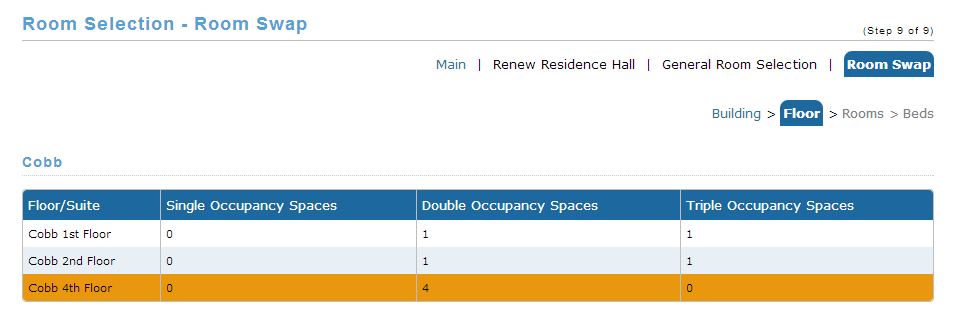
\includegraphics[width=.7\linewidth]{slike/rs8.png} %veličina u odnosu na širinu linije
			\centering
			\caption{Prikaz katova i dostupnih slobodnih soba na pojedinom katu}
			\label{fig:promjene} %label mora biti drugaciji za svaku sliku
		\end{figure}
	
		Još je jedna razlika u odnosu na našu aplikaciju to što nisu sve sobe dostupne svima. Na primjer, postoje 'First Year Experience Buildings' koje su dostupne samo brucošima. Također, sobe s više kreveta podijeljene su po spolu. 
		Nakon izbora kata aplikacija prikazuje tlocrt toga kata sa svim dostupnim sobama. 
		
		\begin{figure}[H]
			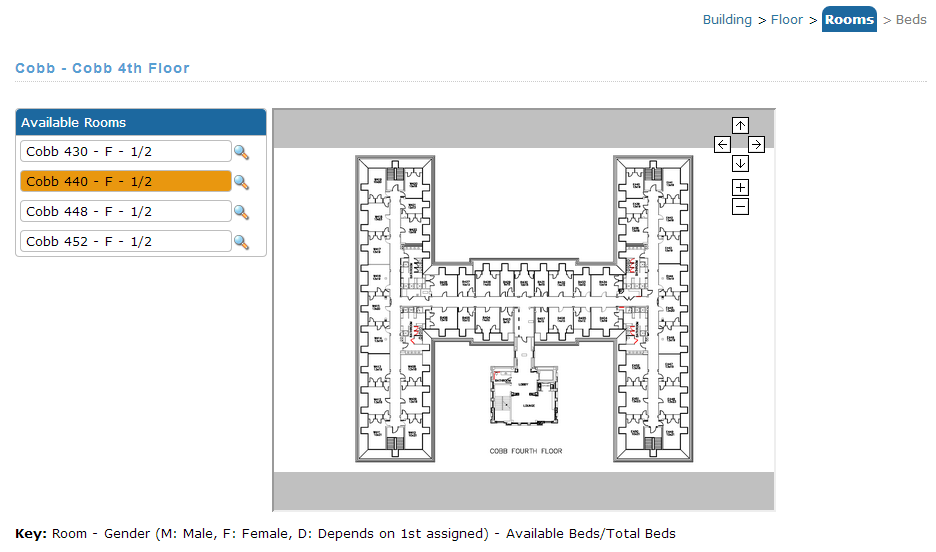
\includegraphics[scale=0.4]{slike/rs9.png} %veličina slike u odnosu na originalnu datoteku i pozicija slike
			\centering
			\caption{Tlocrt odabranog kata}
			\label{fig:promjene2}
		\end{figure}
	
		Klikom na sobu moguć je prikaz detalja o sobi ali i studentu kojemu je trenutno dodijeljena soba. Naša bi aplikacija, uz osnovne informacije o sobi poput doma, paviljona, kata i vrste, nudila i mogućnost detaljnijeg opisa - tip kupaonice, blizina menza itd. 
		
		\begin{figure}[H]
			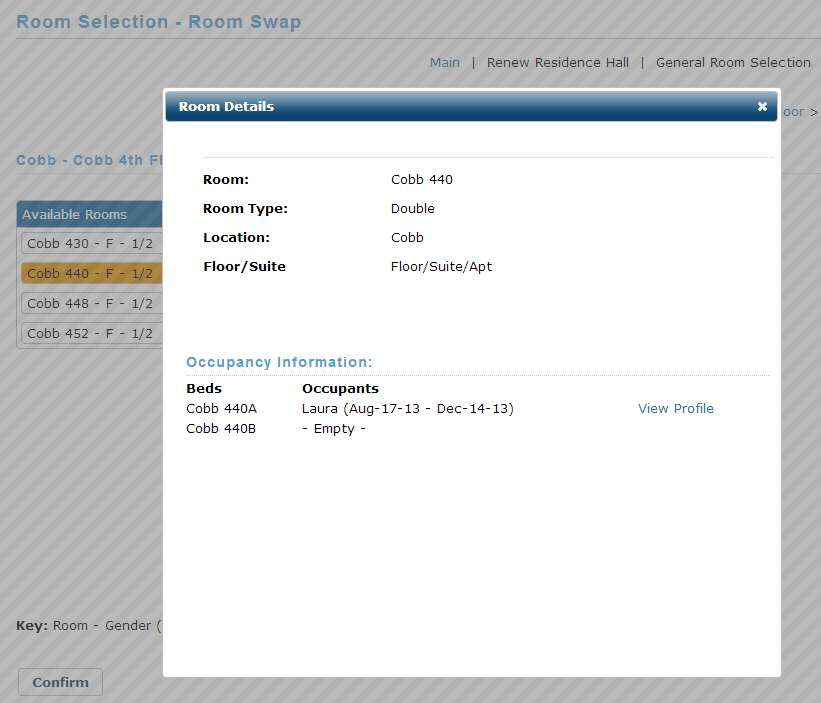
\includegraphics[scale=0.4]{slike/rs10.png} %veličina slike u odnosu na originalnu datoteku i pozicija slike
			\centering
			\caption{Detalji o sobi i studentima u sobi}
			\label{fig:promjene3}
		\end{figure}
	
		Nakon odabira sobe pokreće se odbrojavanje od 5 minuta unutar kojih student mora izabrati krevet u sobi i konačno potvrditi svoj potpuni odabir. Ako se odabir unutar 5 minuta ne potvrdi zamjena se neće provesti. Naša aplikacija ne bi postavljala vremensko ograničenje na potvrdu zamjene, već bi se čekala potvrda obje strane.
		
		\begin{figure}[H]
			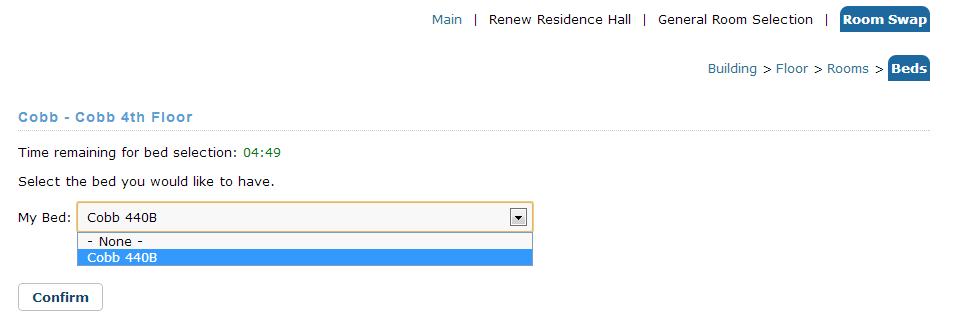
\includegraphics[scale=0.5]{slike/rs11.png} %veličina slike u odnosu na originalnu datoteku i pozicija slike
			\centering
			\caption{Odbrojavanje i konačni odabir}
			\label{fig:promjene4}
		\end{figure}
	
		\clearpage
		
		
		
		\eject
		
	

	\chapter{Specifikacija programske potpore}

\section{Funkcionalni zahtjevi}


\noindent \textbf{Dionici:}

\begin{packed_enum}
	
	\item Studenti
	\item Djelatnici Studentskih centara		
	\item Razvojni tim
	
	
\end{packed_enum}

\noindent \textbf{Aktori i njihovi funkcionalni zahtjevi:}


\begin{packed_enum}
	\item  \underbar{Neregistrirani korisnik (inicijator) može:}
	
	\begin{packed_enum}
		
		\item vidjeti sve oglase
		\item se registrirati, za stvaranje korisničkog računa potrebni su: ime, prezime,korisničko ime, lozinka, e-mail, JMBAG, grad u kojem studira
		
	\end{packed_enum}
	
	\item  \underbar{Registrirani korisnik (inicijator) može:}
	
	\begin{packed_enum}
		
		\item se prijaviti u sustav
		\item stvoriti oglas
		\item vidjeti svoj profil i mijenjati podatke
		\item izbrisati svoj profil
		\item vidjeti oglase pojedinačne ili ulančane koji odgovaraju njegovim kriterijima
		\item pregledati sve svoje oglase (aktivne i neaktivne)
		\item uređivati svoje oglase
		\item učiniti svoje oglase aktivnim i neaktivnim
		\item brisati svoj oglas
		\item "lajkati" oglase po stupnjevima:
		\begin{packed_enum}
			
			\item 1-sviđa mi se
			\item 2-sviđa mi se jako
			\item 3-to je to
			\item Ne prikazuj više ovaj oglas
			
		\end{packed_enum}
		
	\end{packed_enum}
	
	\item  \underbar{Djelatnik SC-a (inicijator) može:}
	
	\begin{packed_enum}
		\item se prijaviti u sustav
		\item pregledati sve zaključane zamjene
	\end{packed_enum}

	\item  \underbar{Timer (inicijator) može:}
	
	\begin{packed_enum}
		\item pokrenuti uparivanje studenata s oglasima koji odgovaraju njegovim kriterijima
		
	\end{packed_enum}
	
	\item  \underbar{Baza podataka (sudionik):}
	
	\begin{packed_enum}
		\item pohranjuje sve podatke o korisnicima i njihovim ovlastima
		\item pohranjuje sve podatke o oglasima i sobama
	\end{packed_enum}
	
	
	\item  \underbar{Poslužitelj (sudionik):}
	
	\begin{packed_enum}
		\item obrađuje zahtjeve korisnika
		
	\end{packed_enum}
	
	
\end{packed_enum}

\eject 



\subsection{Obrasci uporabe}




\noindent \underbar{\textbf{UC1 -Pregled oglasa}}
\begin{packed_item}
	
	\item \textbf{Glavni sudionik: }Neprijavljeni korisnik
	\item  \textbf{Cilj:}Pregledati oglase soba
	\item  \textbf{Sudionici:} baza podataka
	\item  \textbf{Preduvjet:} 
	\item  \textbf{Opis osnovnog tijeka:}
	
	\item[] \begin{packed_enum}
		
		\item Prilikom otvaranja aplikacije sustav prikazuje sve oglase
		
	\end{packed_enum}
	
	
	
	
\end{packed_item}

\noindent \underbar{\textbf{UC2 -Registracija}}
\begin{packed_item}
	
	\item \textbf{Glavni sudionik: }Neregistrirani korisnik
	\item  \textbf{Cilj:}Registrirati korisnika i ovlastiti ga
	\item  \textbf{Sudionici:} baza podataka, poslužitelj
	\item  \textbf{Preduvjet:} dostupnost poslužitelja, korisnik nije registriran
	\item  \textbf{Opis osnovnog tijeka:}
	
	\item[] \begin{packed_enum}
		
		\item Korisnik pritišće tipku "Registracija"
		\item Sustav otvara stranicu za registraciju
		\item Korisnik unosi potrebne podatke
		\item Sustav provjerava ispravnost podataka
		\item Sustav registrira korisnika
		\item Korisnik prima podatke o uspješnoj registraciji
		
	\end{packed_enum}
	
	\item  \textbf{Opis mogućih odstupanja:}
	
	\item[] \begin{packed_item}
		
		\item[2.a]Korisnik unosi neispravne podatke ili već zauzeto korisničko ime ili e-mail
		\item[] \begin{packed_enum}
			
			\item Sustav obavještava korisnika o pogrešci 
			\item Sustav vraća korisnika na stranicu za registraciju sa crveno označenom greškom
			\item Korisnik mijenja neispravne podatke te završava unos ili odustaje od registracije
			
		\end{packed_enum}
		
	\end{packed_item}
\end{packed_item}

\noindent \underbar{\textbf{UC3 -Prijava u sustav}}
\begin{packed_item}
	
	\item \textbf{Glavni sudionik: }Registrirani korisnik, Djelatnik SC-a
	\item  \textbf{Cilj:}Prijaviti se u sustav
	\item  \textbf{Sudionici:} baza podataka
	\item  \textbf{Preduvjet:} Korisnik se je registrirao
	\item  \textbf{Opis osnovnog tijeka:}
	
	\item[] \begin{packed_enum}
		
		\item Unos korisničkog imena i lozinke
		\item Sustav provjerava ispravnost podataka
		\item Sustav korisniku otvara početnu stranicu i korisnik ima pristup korisničkim funkcijama
	\end{packed_enum}
	
	\item  \textbf{Opis mogućih odstupanja:}
	
	\item[] \begin{packed_item}
		
		\item[2.a] Unos neispravnih podataka
		\item[] \begin{packed_enum}
			
			\item  Sustav obavještava o neispravnim podacima i vraća na stanicu za prijavu s crveno označenom pogreškom
			\item Korisnik ispravlja podatke
			
			
		\end{packed_enum}
		
	\end{packed_item}
\end{packed_item}

\noindent \underbar{\textbf{UC4 -Objavljivanje oglasa}}
\begin{packed_item}
	
	\item \textbf{Glavni sudionik: }Prijavljeni korisnik
	\item  \textbf{Cilj:}Objaviti oglas
	\item  \textbf{Sudionici:} baza podataka,poslužitelj
	\item  \textbf{Preduvjet:} Korisnik je prijavljen u sustav
	\item  \textbf{Opis osnovnog tijeka:}
	
	\item[] \begin{packed_enum}
		
		\item Korisnik odabire opciju "Objavi novi oglas"
		\item Sustav otvara stranicu za objavljivanje oglasa
		\item Korisnik upisuje potrebne podatke za sobu koju nudi i kriterije za sobu koju traži. Sve podatke odabire iz padajućih izbornika osim polja za proizvoljni komentar
		\item Korisnik pritišće tipku "objavi" 
		\item Sustav pohranjuje oglas u bazu
	\end{packed_enum}
	
\end{packed_item}

\noindent \underbar{\textbf{UC5 -Pregled mogućih zamjena }}
\begin{packed_item}
	
	\item \textbf{Glavni sudionik: }Prijavljeni korisnik
	\item  \textbf{Cilj:}Pregledati ponuđene moguće zamjene koje odgovaraju kriterijima korisnika
	\item  \textbf{Sudionici:} baza podataka, poslužitelj
	\item  \textbf{Preduvjet:} Korisnik je prijavljen i ima aktivan oglas
	\item  \textbf{Opis osnovnog tijeka:}
	
	\item[] \begin{packed_enum}
		
		\item Korisnik otvara početnu stranicu
		\item Sustav prikazuje sve oglase koji odgovaraju njegovim kriterijima
		
	\end{packed_enum}
\end{packed_item}
\noindent \underbar{\textbf{UC6 - Uparivanje oglasa}}
\begin{packed_item}
	
	\item \textbf{Glavni sudionik: }Timer
	\item  \textbf{Cilj:}Upariti studenta s oglasima koji odgovaraju njegovim kriterijima
	\item  \textbf{Sudionici:} baza podataka, poslužitelj
	\item  \textbf{Preduvjet:}
	\item  \textbf{Opis osnovnog tijeka:}
	
	\item[] \begin{packed_enum}
		
		\item Timer pokreće uparivanje svakih 5 sati
		\item Sustav za svakog studenta stvara listu svih oglasa koji direktno ili lančano odgovaraju njegovim kriterijima
		
	\end{packed_enum}
\end{packed_item}

\noindent \underbar{\textbf{UC7 -Lajkanje oglasa}}
\begin{packed_item}
	
	\item \textbf{Glavni sudionik: }Prijavljeni korisnik
	\item  \textbf{Cilj:}"Lajkati" oglase soba koje korisnika zanimaju
	\item  \textbf{Sudionici:} baza podataka, poslužitelj
	\item  \textbf{Preduvjet:} Korisnik je prijavljen, ima aktivan oglas i barem jedan oglas odgovara njegovim kriterijima
	\item  \textbf{Opis osnovnog tijeka:}
	
	\item[] \begin{packed_enum}
		
		\item Korisnik oglase koji ga zanimaju označava("lajka") po stupnjevima od 1 do 3
		\item Sustav sprema njegov odabir
	\end{packed_enum}
	
\end{packed_item}

\noindent \underbar{\textbf{UC8 -Mjenjanje Lajka}}
\begin{packed_item}
	
	\item \textbf{Glavni sudionik: }Prijavljeni korisnik
	\item  \textbf{Cilj:}Promijeniti razinu "lajka" ili maknuti lajk
	\item  \textbf{Sudionici:} baza podataka, poslužitelj
	\item  \textbf{Preduvjet:} Korisnik je prijavljen, ima aktivan oglas,barem jedan oglas odgovara njegovim kriterijima
	\item  \textbf{Opis osnovnog tijeka:}
	
	\item[] \begin{packed_enum}
		
		\item Korisnik odabire neki drugi stupanj "lajka" ili odustaje od "lajka" micanjem oznake
		\item Njegov odabir se sprema u bazu podataka
		
	\end{packed_enum}
	
\end{packed_item}

\noindent \underbar{\textbf{UC9 -Pregled mojih oglasa}}
\begin{packed_item}
	
	\item \textbf{Glavni sudionik: }Prijavljeni korisnik
	\item  \textbf{Cilj:}Vidjeti sve svoje oglase
	\item  \textbf{Sudionici:} baza podataka, poslužitelj
	\item  \textbf{Preduvjet:} Korisnik je prijavljen i ima oglas
	\item  \textbf{Opis osnovnog tijeka:}
	
	\item[] \begin{packed_enum}
		
		\item Korisnik odabire opciju "Moji oglasi"
		\item Sustav otvara stranicu gdje se prikazuju svi korisnikovi oglasi
		
	\end{packed_enum}
\end{packed_item}

\noindent \underbar{\textbf{UC10 -Uređivanje oglasa}}
\begin{packed_item}
	
	\item \textbf{Glavni sudionik: }Prijavljeni korisnik
	\item  \textbf{Cilj:}Urediti već postojeći oglas
	\item  \textbf{Sudionici:} baza podataka, poslužitelj
	\item  \textbf{Preduvjet:} Korisnik je prijavljen i ima aktivan oglas
	\item  \textbf{Opis osnovnog tijeka:}
	
	\item[] \begin{packed_enum}
		
		\item Korisnik odlazi pod "Moji oglasi" 
		\item Sustav prikazuje stranicu sa listom njegovih oglasa
		\item Korisnik odabire opciju uredi
		\item Korisnik mijenja podatke ili atribut je li oglas aktivan ili neaktivan
		\item Korisnik potvrđuje promjene odabirom opcije spremi
		\item Promjene se spremaju u bazu podataka 
		
	\end{packed_enum}
\end{packed_item}



\noindent \underbar{\textbf{UC11 -Brisanje oglasa}}
\begin{packed_item}
	
	\item \textbf{Glavni sudionik: }Prijavljeni korisnik
	\item  \textbf{Cilj:}Izbrisati oglas
	\item  \textbf{Sudionici:} baza podataka, poslužitelj
	\item  \textbf{Preduvjet:} Korisnik je prijavljen i ima oglas
	\item  \textbf{Opis osnovnog tijeka:}
	
	\item[] \begin{packed_enum}
		
		\item Korisnik odlazi pod "Moji oglasi" 
		\item Sustav prikazuje stranicu sa listom njegovih oglasa
		\item Korisnik odabire opciju izbriši
		\item Sustav briše oglas iz baze podataka
		
	\end{packed_enum}
\end{packed_item}

\noindent \underbar{\textbf{UC12 -Pregled profila}}
\begin{packed_item}
	
	\item \textbf{Glavni sudionik: }Prijavljeni korisnik
	\item  \textbf{Cilj:}Vidjeti svoje osobne podatke
	\item  \textbf{Sudionici:} baza podataka, poslužitelj
	\item  \textbf{Preduvjet:} Korisnik je prijavljen
	\item  \textbf{Opis osnovnog tijeka:}
	
	\item[] \begin{packed_enum}
		
		\item Korisnik odlazi pod "Moj profil"
		\item Sustav otvara stranicu korisnikova profila 
		
	\end{packed_enum}
\end{packed_item}

\noindent \underbar{\textbf{UC13 -Promjena profila}}
\begin{packed_item}
	
	\item \textbf{Glavni sudionik: }Prijavljeni korisnik
	\item  \textbf{Cilj:}Vidjeti svoje osobne podatke
	\item  \textbf{Sudionici:} baza podataka, poslužitelj
	\item  \textbf{Preduvjet:} Korisnik je prijavljen
	\item  \textbf{Opis osnovnog tijeka:}
	
	\item[] \begin{packed_enum}
		
		\item Korisnik odlazi pod "Moj profil"
		\item Sustav otvara stranicu korisnikova profila 
		\item Korisnik odabire opciju "uredi"
		\item Korisnik mijenja osobne podatke
		\item Korisnik pritišće tiku "spremi promjene"
		\item Sustav sprema promjene 
		
	\end{packed_enum}
\end{packed_item}

\noindent \underbar{\textbf{UC14 -Brisanje profila}}
\begin{packed_item}
	
	\item \textbf{Glavni sudionik: }Prijavljeni korisnik
	\item  \textbf{Cilj:}Vidjeti svoje osobne podatke
	\item  \textbf{Sudionici:} baza podataka, poslužitelj
	\item  \textbf{Preduvjet:} Korisnik je prijavljen
	\item  \textbf{Opis osnovnog tijeka:}
	
	\item[] \begin{packed_enum}
		
		\item Korisnik odlazi pod "Moj profil"
		\item Sustav otvara stranicu korisnikova profila 
		\item Korisnik odabire opciju "izbriši profil"
		\item Sustav briše korisnikov profil i otvara početnu stranicu
		
	\end{packed_enum}
\end{packed_item}

\noindent \underbar{\textbf{UC15 -Potvrđivanje zamjene}}
\begin{packed_item}
	
	\item \textbf{Glavni sudionik: }Prijavljeni korisnik
	\item  \textbf{Cilj:}Potvrditi zamjenu sobe
	\item  \textbf{Sudionici:} baza podataka, poslužitelj
	\item  \textbf{Preduvjet:} Korisnik je prijavljen, sve uključene strane su "lajkale" oglas
	\item  \textbf{Opis osnovnog tijeka:}
	
	\item[] \begin{packed_enum}
		
		\item Korisnik dobiva obavijest da su sve strane "lajkale" zamjenu
		\item Korisnik pomoću linka iz obavijesti dolazi do oglasa
		\item Korisnik potvrđuje zamjenu
		\item Potvrda se sprema u bazu podataka
		
	\end{packed_enum}
\end{packed_item}
\noindent \underbar{\textbf{UC16 -Pregled zaključanih zamjena}}
\begin{packed_item}
	
	\item \textbf{Glavni sudionik: }Djelatnik SC-a
	\item  \textbf{Cilj:}Vidjeti sve zaključane zamjene kako bi se mogle provesti u sustavu SC-a
	\item  \textbf{Sudionici:} baza podataka, poslužitelj
	\item  \textbf{Preduvjet:}Djelatnik je prijavljen
	\item  \textbf{Opis osnovnog tijeka:}
	
	\item[] \begin{packed_enum}
		
		\item Sustav na početnoj stranici prikazuje listu svih zaključanih zamjena
		\item Korisnik označuje sve zamjene koje je proveo
		\item Sustav miče označene zamjene sa stranice
		
		
	\end{packed_enum}
	
\end{packed_item}	
\noindent \underbar{\textbf{UC17 -Odjava}}
\begin{packed_item}
	
	\item \textbf{Glavni sudionik: }Djelatnik SC-a, Prijavljeni korisnik
	\item  \textbf{Cilj:}Odjaviti se iz sustava
	\item  \textbf{Sudionici:}poslužitelj
	\item  \textbf{Preduvjet:}Djelatnik je prijavljen
	\item  \textbf{Opis osnovnog tijeka:}
	
	\item[] \begin{packed_enum}
		
		\item Korisnik pritišće tipku "odjavi se"
		\item Sustav odjavljuje korisnika te otvara početnu stranicu		
		
	\end{packed_enum}
	
\end{packed_item}	

\noindent \textbf{Dijagrami obrazaca uporabe}
\begin{figure}[H]
	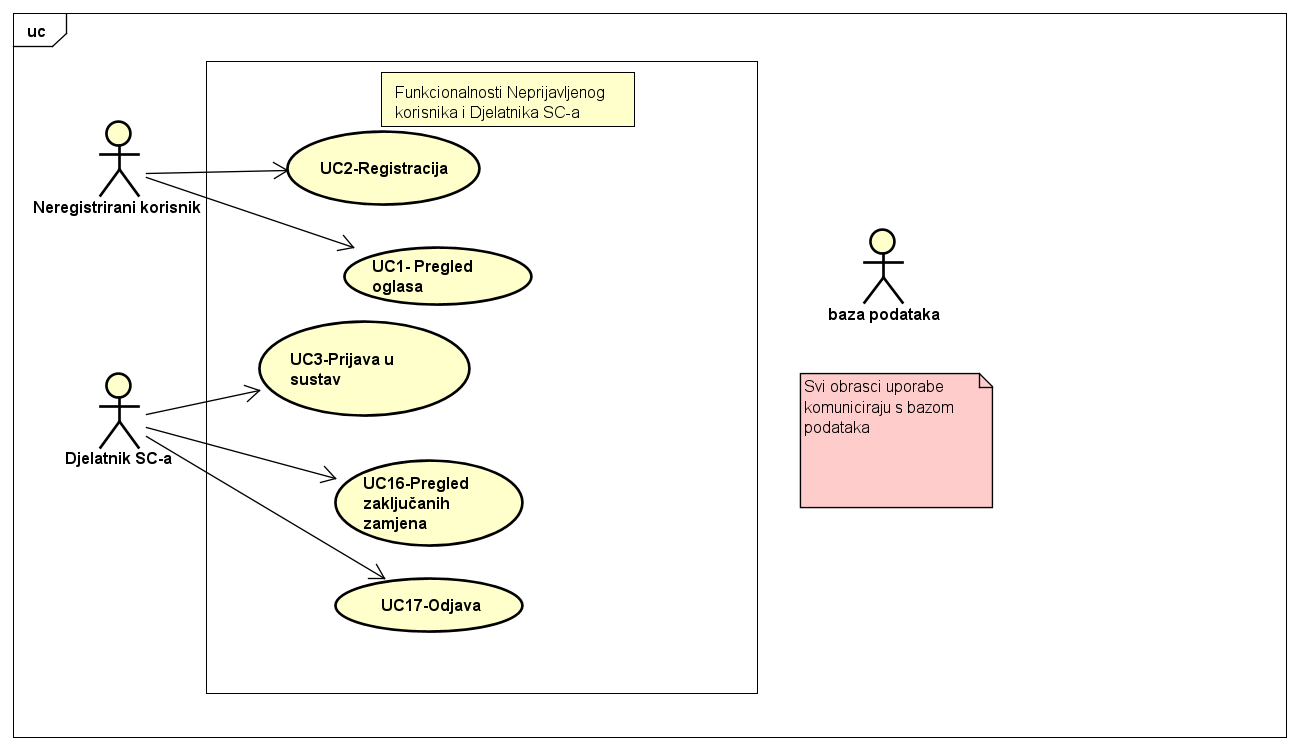
\includegraphics[scale=0.4]{dijagrami/dijagram1.PNG} %veličina slike u odnosu na originalnu datoteku i pozicija slike
	\centering
	\caption{Dijagrami obrazaca uporabe, funkcionalnost neregistriranog korisnika i djelatnika SC-a}
	\label{fig:dijagramObrazaca1}
\end{figure}

\begin{figure}[H]
	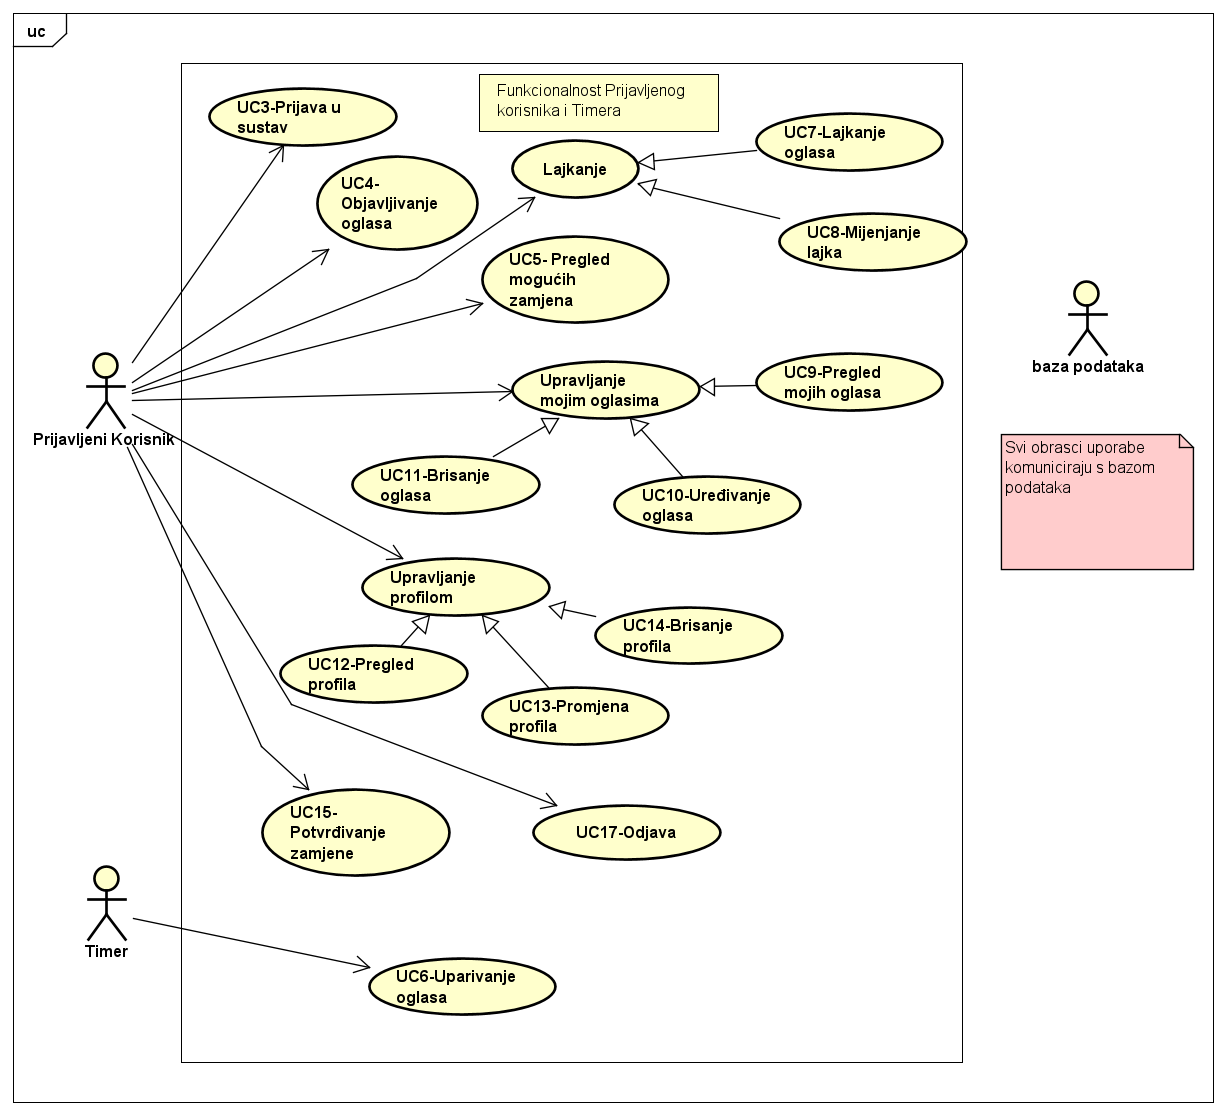
\includegraphics[scale=0.4]{dijagrami/dijagram2.PNG} %veličina slike u odnosu na originalnu datoteku i pozicija slike
	\centering
	\caption{Dijagrami obrazaca uporabe, funkcionalnost prijavljenog korisnika i timera}
	\label{fig:dijagramObrazaca2}
\end{figure}

\eject

\subsection{Sekvencijski dijagrami}

\noindent \textbf{Obrazac uporabe UC3(Prijava u sustav)}\\
	\indent Neprijavljeni korisnik šalje zahtjev za prijavu s korisničkim imenom i lozinkom. Provjerava se ako je korisničko ime u bazi podataka. Ako ime ne postoji dojavljuje se greška u suprotnom provjerava se ako mu odgovara unesena lozinka. Ako lozinka odgovara tada se korisniku dodjeljuju ovlasti u suprotnom se dojavljuje greška.


\begin{figure}[H]
	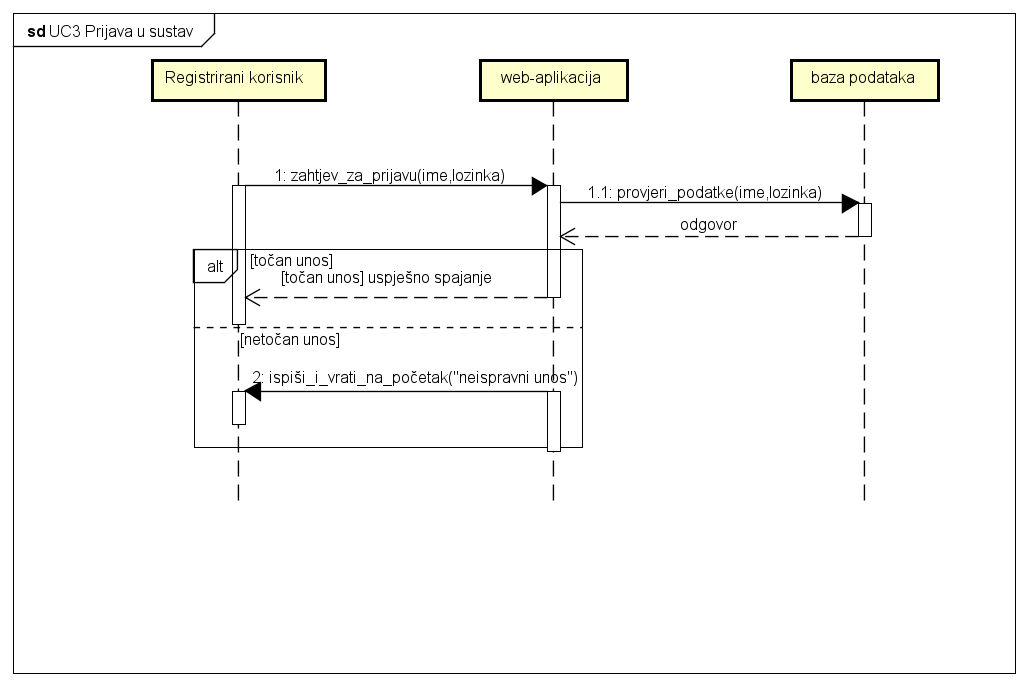
\includegraphics[scale=0.4]{dijagrami/UC3 Prijava u sustav.PNG} %veličina slike u odnosu na originalnu datoteku i pozicija slike
	\centering
	\caption{Sekvencijski dijagram za UC3}
	\label{fig:sekdijag1}
\end{figure}

\noindent \textbf{Obrazac uporabe UC4(Objavljivanje oglasa)}\\
\indent Korisnik odabire opciju "Objavi novi oglas". Zatim u obrascu iz padajućih izbornika bira grad zatim mu se nude svi domovi. Nakon odabira doma prikazuju mu se paviljoni i tako dalje za kat i broj sobe. Zatim korisnik označava iste  kriterije za sobu koju traži. Pritiskom na oznaku spremi sprema se oglas u bazu podataka.



\begin{figure}[H]
	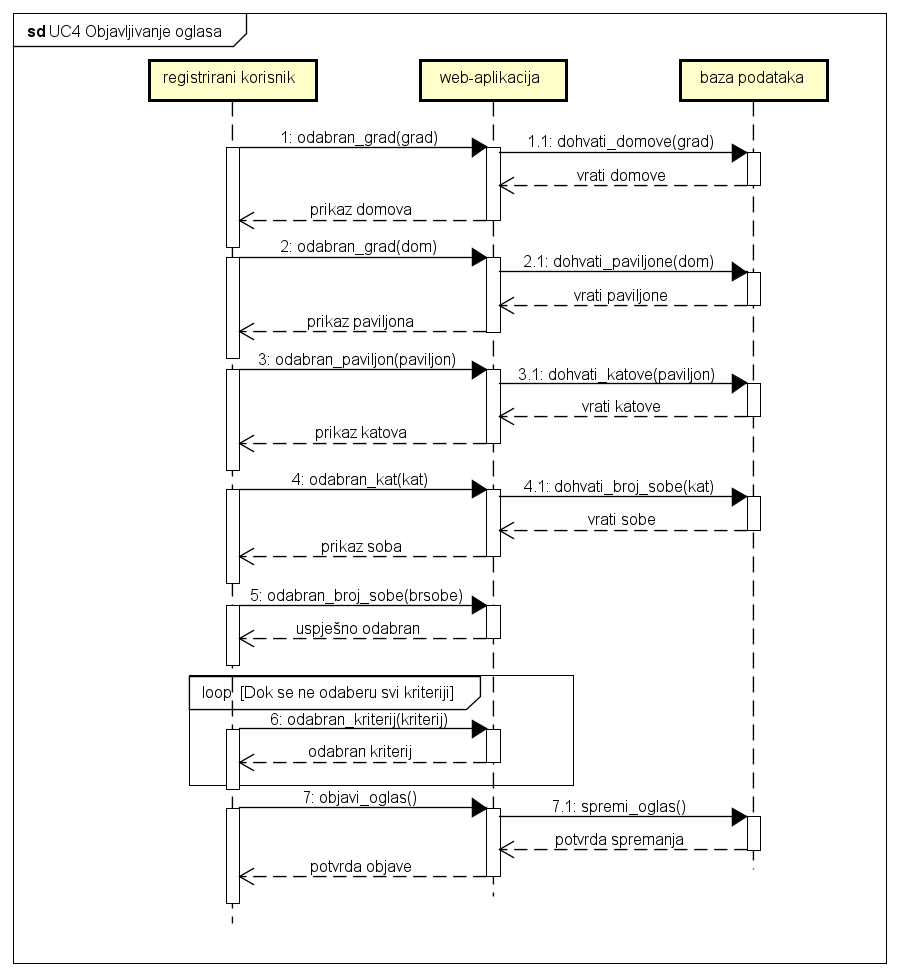
\includegraphics[scale=0.4]{dijagrami/UC4 Objavljivanje oglasa.PNG} %veličina slike u odnosu na originalnu datoteku i pozicija slike
	\centering
	\caption{Sekvencijski dijagram za UC4}
	\label{fig:sekdijag2}
\end{figure}

\noindent \textbf{Obrazac uporabe UC5(Pregled mogućih zamjena)}\\
\indent Korisnik nakon što napravi oglas odlazi na početnu stranicu gdje dobiva listu svih oglasa koji odgovaraju njegovim kriterijima.


\begin{figure}[H]
	\includegraphics[scale=0.4]{dijagrami/UC5 Pregled mogućih zamjena.PNG} %veličina slike u odnosu na originalnu datoteku i pozicija slike
	\centering
	\caption{Sekvencijski dijagram za UC5}
	\label{fig:sekdijag3}
\end{figure}

\noindent \textbf{Obrazac uporabe UC15(Potvrđivanje zamjene)}\\
\indent Korisnik potvrđuje zamjenu odabirom opcije "zaključaj zamjenu". Potvrda se sprema u bazu podataka promjenom statusa oglasa tek kad sve strane potvrde zamjenu.


\begin{figure}[H]
	\includegraphics[scale=0.4]{dijagrami/UC15 Potvrđivanje zamjene.PNG} %veličina slike u odnosu na originalnu datoteku i pozicija slike
	\centering
	\caption{Sekvencijski dijagram za UC15}
	\label{fig:sekdijag4}
\end{figure}

\section{Ostali Zahtjevi}
\begin{packed_enum}
	\item Sustav treba omogućiti rad više korisnika u stvarnom vremenu
	\item Sustav bi se trebao moći koristiti bez dodatnih uputa
	\item Sustav i korisničko sučelje trebaju podržavati hrvatsku abecedu
	\item Izvršavanje dijela programa u kojem se pristupa bazi podataka ne smije trajati duže od nekoliko sekundi
	\item Neispravno korištenje korisničkog sučelja ne smije narušiti funkcionalnost i rad sustava
	\item Nadogradnja sustava ne smije narušavati postojeće funkcionalnosti sustava
	\item Aplikacija treba biti izvedena kao web aplikacija prilagođena (engl. responsive) mobilnom uređaju
\end{packed_enum}




	\chapter{Arhitektura i dizajn sustava}
		
			Arhitektura sustava je web aplikacija kojoj će korisnici pristupati pomoću web preglednika. Odlučili smo se na takvu arhitekturu jer je cilj sustava da bude što jednostavniji za korištenje i da mu se može pristupiti sa svih mjesta.
			
			\begin{figure}[H]
				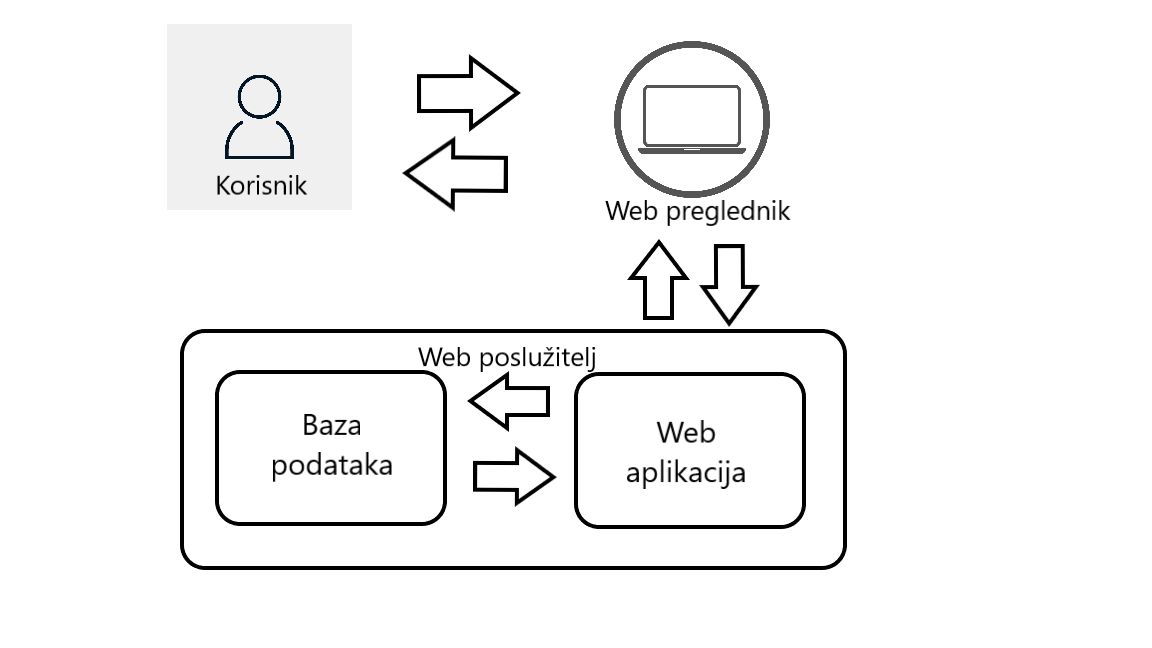
\includegraphics[scale=0.4]{slike/Skica_sustava.png} %veličina slike u odnosu na originalnu datoteku i pozicija slike
				\centering
				\caption{Skica sustava}
				\label{fig:sustav}
			\end{figure}
			
			Programski jezik koji smo odabralni za izradu aplikacije je java s razvojnim okvirom Spring Boot te javaScript. Odabrano razvojno okruženje je IntelliJ IDEA. 
			Aplikacija je organizirana u dva sloja: frontend i backend. Za izradu frontenda koristi se React.React je javaScript biblioteka koja služi za izradu jednostranične aplikacije. Frontend i backend komuniciraju pomoću RESTa. REST se bazira na HTTP protokolu. Backend se sastoji od pet komponenti:
		\begin{itemize}
		\item Kontroler - služi za komunikaciju s frontendom. Zaprima HTTP zathtjev te određuje koja će se funkcionalnost izvršavati
		\item Servis - u njima se odvijaju poslovne logike i sve funkcionalnosti aplikacije
		\item Repozitorij - dohvaća i sprema podatke u bazu podataka
		\item Model - opisuju entitete iz baze 
		\item Security - omogućava autentikaciju i autorizaciju 
	\end{itemize}

\begin{figure}[H]
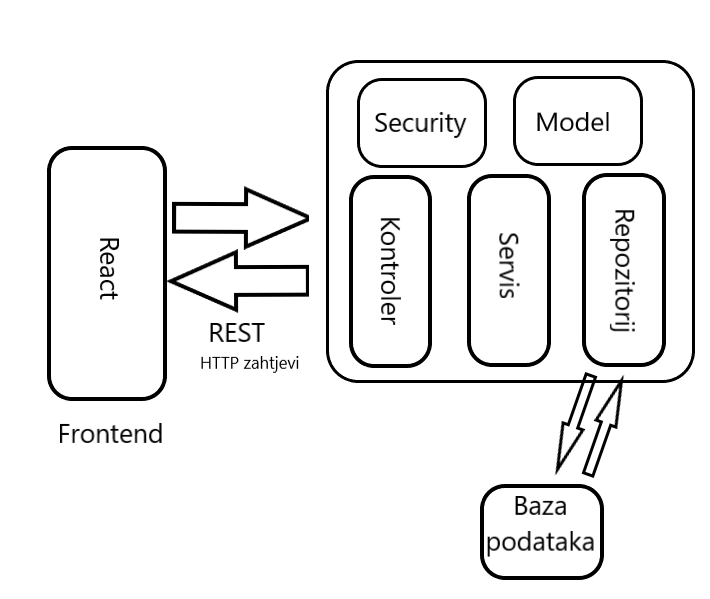
\includegraphics[scale=0.4]{slike/Skica_aplikacije.png} %veličina slike u odnosu na originalnu datoteku i pozicija slike
\centering
\caption{Skica aplikacije}
\label{fig:aplikacija}
\end{figure}


	
		

		

				
		\section{Baza podataka}
			
		Za potrebe sustava za zamjenu soba koristit ćemo relacijsku bazu podataka koja nam omogućuje oblikovanje objekata iz stvarnog svijeta pomoću povezanih tablica - relacija. Svaka je tablica definirana vlastitim nazivom i skupom različitih atributa koji je opisuju. Glavna je zadaća baze podataka pohrana, brzo pronalaženje i dohvaćanje te dodavanje i brisanje podataka. Baza podataka ovog sustava sastoji se od entiteta:
		\begin{itemize}
			\item Student
			\item Oglas
			\item Soba
			\item Grad
			\item Dom
			\item Paviljon
			\item StudentskiCentar
			\item Obavijest
			\item Zaposlenik SC
			\item TrazeniUvjeti
			\item Lajkovi
			\item StudentObavijesti
			
		\end{itemize}
		
			\subsection{Opis tablica}
			

			\textbf{Student } Entitet sadrži informacije o korisniku aplikacije - studentu. Sadrži sljedeće atribute: identifikator studenta, korisničko ime, ime, prezime, e-mail adresu, JMBAG, lozinku te oznaku za primanje mailova. Entitet je u vezi \textit{Many-to-Many} s entitetom Obavijest preko identifikatora obavijesti, u vezi \textit{One-to-One} s entitetom Oglas preko atributa statusa oglasa, u vezi \textit{One-to-One} s entitetom TrazeniUvjeti preko atributa identifikatora uvjeta te u vezi \textit{One-to-One} s entitetom Oglas. 
				
				
				
				\begin{longtabu} to \textwidth {|X[6, 2]|X[6, 2]|X[20, l]|}
					
					\hline \multicolumn{3}{|c|}{\textbf{Student}}	 \\[3pt] \hline
					\endfirsthead
					
					\hline \multicolumn{3}{|c|}{\textbf{Student}}	 \\[3pt] \hline
					\endhead
					
					\hline 
					\endlastfoot
					
					\textbf{idKorisnik} & UUID	& jedinstveni identifikator studenta (korisnika) 	\\ \hline
					korisnickoIme	& VARCHAR & jedinstveno korisničko ime  	\\ \hline 
					jmbag & VARCHAR & jedinstveni JMBAG studenta \\ \hline 
					ime & VARCHAR & ime studenta 		\\ \hline
					prezime & VARCHAR & prezime studenta \\ \hline
					email & VARCHAR & e-mail adresa studenta \\ \hline
					hashLozinke & VARCHAR & hash lozinka \\ \hline
					obavijestiNaMail & BOOLEAN & oznaka želi li student primati obavijesti na mail \\ \hline
					viseOvlasti & BOOLEAN & aa \\ \hline
					\textit{idStatusOglasa} & BOOLEAN & oznaka potvrde \\ \hline
					\textit{idTrazeniUvjeti} & VARCHAR & traženi kriteriji za sobu za zamjenu \\ \hline
				 
					
				\end{longtabu}
			
				\textbf{Oglas } Entitet sadrži informacije koje su vezane uz oglas koji student predaje. Sadrži atribute: ID oglasa, naslov oglasa, opis te datum objave oglasa. Entitet je u vezi \textit{One-to-One} s entitetom Status preko atributa identifiaktora statusa oglasa i u vezi \textit{One-to-Many} s entitetom Obavijest preko atributa identifikatora oglasa.
			
				\begin{longtabu} to \textwidth {|X[6, 2]|X[6, 2]|X[20, l]|}
					
					\hline \multicolumn{3}{|c|}{\textbf{Oglas}}	 \\[3pt] \hline
					\endfirsthead
					
					\hline \multicolumn{3}{|c|}{\textbf{Oglas}}	 \\[3pt] \hline
					\endhead
					
					\hline 
					\endlastfoot
					
					\textbf{idOglas} & UUID	& jedinstveni identifikator oglasa 	\\ \hline
					naslov	& VARCHAR & naslov oglasa  	\\ \hline 
					opis & VARCHAR & opis oglasa \\ \hline 
					objavljen & DATE & datum objavljivanja oglasa 		\\ \hline
					godina & INTEGER & godina objavljivanja oglasa \\ \hline
					\textit{idStatusOglasa} & VARCHAR & status oglasa \\ \hline
					
					 
					
					
				\end{longtabu}
			
				\textbf{Soba } Entitet sadrži informacije o sobi u studentskom domu. Sadrži atribute: broj sobe, kat na kojemu se soba nalazi,broj kreveta i vrstu kupaonice koja pripada sobi, kategoriju te identifikator paviljona i doma. Entitet je u vezi \textit{Many-to-One} s entitetom Paviljon preko atributa identifikatora paviljona i doma.
			
				\begin{longtabu} to \textwidth {|X[6, 2]|X[6, 2]|X[20, l]|}
					
					\hline \multicolumn{3}{|c|}{\textbf{Soba}}	 \\[3pt] \hline
					\endfirsthead
					
					\hline \multicolumn{3}{|c|}{\textbf{Soba}}	 \\[3pt] \hline
					\endhead
					
					\hline 
					\endlastfoot
					
					\textbf{broj} & INTEGER & broj sobe 	\\ \hline
					\textbf{kat} & INTEGER & kat na kojemu se soba nalazi \\ \hline 
					brojKreveta & VARCHAR & broj kreveta u sobi \\ \hline
					tipKupaonice & VARCHAR & vrsta dostupne kupaonice \\ \hline
					kategorija & VARCHAR & kategorija sobe \\ \hline
					\textbf{\textit{idPaviljon}} & UUID & identifikator paviljona kojemu soba pripada \\ \hline
					\textbf{\textit{idDom}} & UUID & identifikator doma kojemu soba pripada \\ \hline
					
					
				\end{longtabu}
			
				\textbf{Grad } Entitet sadrži informacije o pojedinom gradu. Sadrži atribute: identifikator grada i naziv te identifikator studentskog centra tog grada. Entitet je u vezi \textit{One-To-One} s entitetom Studentski Centar preko atributa identifikatora studentskog centra i u vezi \textit{One-to-Many} s entitetom Dom preko identifikatora grada. 
			
				\begin{longtabu} to \textwidth {|X[6, 2]|X[6, 2]|X[20, l]|}
					
					\hline \multicolumn{3}{|c|}{\textbf{Grad}}	 \\[3pt] \hline
					\endfirsthead
					
					\hline \multicolumn{3}{|c|}{\textbf{Grad}}	 \\[3pt] \hline
					\endhead
					
					\hline 
					\endlastfoot
					
					\textbf{idGrad} & UUID	& jedinstveni identifikator grada	\\ \hline
					naziv	& VARCHAR & ime grada  	\\ \hline  
					\textit{idSc} & UUID & identifikator gradskog studentskog centra \\ \hline
					
					
				\end{longtabu}
			
				\textbf{Dom } Entitet sadrži sve važne informacije o pojedinom studentskom domu. Sadrži atribute: ID doma, naziv doma, ID grada u kojemu se dom nalazi te oznaku ima li dom vlastitu menzu. Entitet je u vezi \textit{Many-to-One} s entitetom Grad preko atributa identifikatora grada i u vezi \text{One-To-Many} s entitetom Paviljon preko identifikatora doma. 
			
				\begin{longtabu} to \textwidth {|X[6, 2]|X[6, 2]|X[20, l]|}
					
					\hline \multicolumn{3}{|c|}{\textbf{Dom}}	 \\[3pt] \hline
					\endfirsthead
					
					\hline \multicolumn{3}{|c|}{\textbf{Dom}}	 \\[3pt] \hline
					\endhead
					
					\hline 
					\endlastfoot
					
					\textbf{idDom} & UUID	& jedinstveni identifikator studentskog doma 	\\ \hline
					naziv	& VARCHAR & ime studentskog doma  	\\ \hline 
					imaMenzu & BOOLEAN & oznaka ima li dom vlastitu menzu \\ \hline
					\textit{idGrad} & UUID & identifikator grada u kojemu se dom nalazi \\ \hline
					
					
				\end{longtabu}
			
				\textbf{Paviljon } Entitet sadrži sve informacije o pojedinom paviljonu studentskog doma. Sadrži atribute: identifikator paviljona, naziv te identifikator doma. Entitet je u vezi \textit{Many-to-One} s entitetom Dom preko atributa identifikatora doma te u vezi \textit{One-to-Many} s entitetom Soba preko indetifikatora paviljona. 
			
				\begin{longtabu} to \textwidth {|X[6, 2]|X[6, 2]|X[20, l]|}
					
					\hline \multicolumn{3}{|c|}{\textbf{Paviljon}}	 \\[3pt] \hline
					\endfirsthead
					
					\hline \multicolumn{3}{|c|}{\textbf{Paviljon}}	 \\[3pt] \hline
					\endhead
					
					\hline 
					\endlastfoot
					
					\textbf{idPaviljon} & UUID	& jedinstveni identifikator paviljona	\\ \hline
					naziv & VARCHAR & naziv paviljona  	\\ \hline 
					\textit{idDom} & UUID & identifikator doma u kojemu se paviljon nalazi \\ \hline
					
					
				\end{longtabu}
			
			
				\textbf{Studentski centar } Entitet sadrži informacije o studentskom centru. Sadrži atribute: identifikator studentskog centra, naziv te identifikator grada u kojemu se studentski centar nalazi. Entitet je u vezi \textit{One-to-One} s entitetom Grad preko atributa identifikatora grada te u vezi \textit{One-to-Many} s entitetom Zaposlenik SC preko identifikatora studentskog centra. 
			
				\begin{longtabu} to \textwidth {|X[6, 2]|X[6, 2]|X[20, l]|}
					
					\hline \multicolumn{3}{|c|}{\textbf{Studentski Centar}}	 \\[3pt] \hline
					\endfirsthead
					
					\hline \multicolumn{3}{|c|}{\textbf{Studentski centar}}	 \\[3pt] \hline
					\endhead
					
					\hline 
					\endlastfoot
					
					\textbf{idSc} & UUID & jedinstveni identifikator studentskog centra	\\ \hline
					naziv  & VARCHAR & ime studentskog centra  	\\ \hline
					\textit{idGrad} & UUID & identifikator grada u kojemu se nalazi studentski centar \\ \hline
					
					
				\end{longtabu}
			
				\textbf{Obavijest} Entitet sadrži informacije o obavijestima koje aplikacija šalje studentima. Sadrži entitete: identifikator obavijesti, tekst, oznaku je li obavijest procitana, vrijeme slanja obavijesti te listu studenata kojima se obavijest šalje i identifikator oglasa za koji se obavijest šalje. Entitet je u vezi \textit{Many-to-Many} s entitetom Student te u vezi \textit{Many-to-One} s entitetom Oglas preko identifikatora oglasa. 
			 
				\begin{longtabu} to \textwidth {|X[6, 2]|X[6, 2]|X[20, l]|}
					
					\hline \multicolumn{3}{|c|}{\textbf{Obavijest}}	 \\[3pt] \hline
					\endfirsthead
					
					\hline \multicolumn{3}{|c|}{\textbf{Obavijest}}	 \\[3pt] \hline
					\endhead
					
					\hline 
					\endlastfoot
					
					\textbf{idObavijest} & UUID & jedinstveni identifikator obavijesti	\\ \hline
					tekst  & VARCHAR & tekst obavijesti  	\\ \hline 
					procitana & BOOLEAN & oznaka je li poruka pročitana \\ \hline
					vrijeme & DATE & vrijeme slanja obavijesti \\ \hline
					\textit{idOglas} & UUID & identifikator oglasa za koji se obavijest generira \\ \hline
					
					
				\end{longtabu}
			
				\textbf{Zaposlenik SC } Entitet sadrži informacije o zaposleniku u studentskom centru. Sadrži atribute: identifikator zaposlenika, korisničko ime i lozinku za prijavu u sustav, ime i prezime zaposlenika, e-mail adresu te identifikator studentskog centra u kojem je zaposlen.
			
				\begin{longtabu} to \textwidth {|X[6, 2]|X[6, 2]|X[20, l]|}
					
					\hline \multicolumn{3}{|c|}{\textbf{Zaposlenik SC}}	 \\[3pt] \hline
					\endfirsthead
					
					\hline \multicolumn{3}{|c|}{\textbf{Zaposlenik SC}}	 \\[3pt] \hline
					\endhead
					
					\hline 
					\endlastfoot
					
					\textbf{idZaposlenik} & UUID	& jedinstveni identifikator zaposlenika studentskog centra	\\ \hline
					korisnickoIme & VARCHAR & jedinstveno korisničko ime zaposlenika studentskog centra \\ \hline
					ime & VARCHAR & ime zaposlenika studentskog centra \\ \hline
					prezime & VARCHAR & prezime zaposlenika studentskog centra \\ \hline
					email & VARCHAR & e-mail adresa zaposlenika studentskog centra \\ \hline
					hashLozinke & VARCHAR & hash lozinke \\ \hline
					\textit{idSc} & UUID & identifikator studentskog centra u kojemu je zaposlen \\ \hline
				
					
					
				\end{longtabu}
			
				\begin{longtabu} to \textwidth {|X[6, 2]|X[6, 2]|X[20, l]|}
					
					\hline \multicolumn{3}{|c|}{\textbf{TrazeniUvjeti}}	 \\[3pt] \hline
					\endfirsthead
					
					\hline \multicolumn{3}{|c|}{\textbf{TrazeniUvjeti}}	 \\[3pt] \hline
					\endhead
					
					\hline 
					\endlastfoot
					
					\textbf{idTrazeniUvjeti} & UUID	& jedinstveni identifikator skupa traženih uvjeta	\\ \hline
					brojKreveta & VARCHAR & traženi broj kreveta \\ \hline
					tipKupaonice & VARCHAR & traženi tip kupaonice \\ \hline
					kateogrija & VARCHAR & tražena kategorija \\ \hline
					godina & INTEGER & godina za koju se predaje oglas \\ \hline
					komentar & VARCHAR & dodatni komentari vezani uz tražene uvjete \\ \hline
					
					
					
					
					
				\end{longtabu}
			
				\textbf{Lajkovi} Entitet sadrži informacije vezane uz 'lajkove' oglasa. Sadrži atribute: identifikator oglasa i identifikator studenta te ocjenu. Entitet je u vezi \textit{Many-to-One} s entitetom Student preko identifikatora studenta i u vezi \textit{Many-to-One} s entitetom Oglas preko identifikatora oglasa.
			
				\begin{longtabu} to \textwidth {|X[6, 2]|X[6, 2]|X[20, l]|}
					
					\hline \multicolumn{3}{|c|}{\textbf{Lajkovi}}	 \\[3pt] \hline
					\endfirsthead
					
					\hline \multicolumn{3}{|c|}{\textbf{Lajkovi}}	 \\[3pt] \hline
					\endhead
					
					\hline 
					\endlastfoot
					
					\textbf{idOglas} & UUID & jedinstveni identifikator oglasa koji se ocjenjuje \\ \hline
					\textbf{idStudent} & UUID & jedinstveni identifikator studenta koji je 'dao lajk' \\ \hline
					ocjena & INTEGER & iznos ocjene \\ \hline
					
					
				\end{longtabu}
			
				\begin{longtabu} to \textwidth {|X[6, 2]|X[6, 2]|X[20, l]|}
					
					\hline \multicolumn{3}{|c|}{\textbf{Status oglasa}}	 \\[3pt] \hline
					\endfirsthead
					
					\hline \multicolumn{3}{|c|}{\textbf{Status oglasa}}	 \\[3pt] \hline
					\endhead
					
					\hline 
					\endlastfoot
					
					\textbf{idStautsOglasa} & UUID & jedinstveni identifikator statusa oglasa \\ \hline
					status & INTEGER & aa \\ \hline
					\textit{idOglas} & UUID & identifikator oglasa\\ \hline
					\textit{idStudent} & UUID & identifikator studenta \\ \hline
					
					
					
					
				\end{longtabu}
			
				\begin{longtabu} to \textwidth {|X[6, 2]|X[6, 2]|X[20, l]|}
					
					\hline \multicolumn{3}{|c|}{\textbf{StudentObavijesti}}	 \\[3pt] \hline
					\endfirsthead
					
					\hline \multicolumn{3}{|c|}{\textbf{StudentObavijesti}}	 \\[3pt] \hline
					\endhead
					
					\hline 
					\endlastfoot
					
					\textit{studentiIdKorisnik} & UUID & aa \\ \hline
					\textit{obavijestiIdObavijest} & UUID & aa \\ \hline
					
					
					
					
				\end{longtabu}
			
				\begin{longtabu} to \textwidth {|X[6, 2]|X[6, 2]|X[20, l]|}
					
					\hline \multicolumn{3}{|c|}{\textbf{Broj kreveta}}	 \\[3pt] \hline
					\endfirsthead
					
					\hline \multicolumn{3}{|c|}{\textbf{Broj kreveta}}	 \\[3pt] \hline
					\endhead
					
					\hline 
					\endlastfoot
					
					
					
					
				\end{longtabu}
			
				\begin{longtabu} to \textwidth {|X[6, 2]|X[6, 2]|X[20, l]|}
					
					\hline \multicolumn{3}{|c|}{\textbf{Oznake kategorija}}	 \\[3pt] \hline
					\endfirsthead
					
					\hline \multicolumn{3}{|c|}{\textbf{Oznake kategorija}}	 \\[3pt] \hline
					\endhead
					
					\hline 
					\endlastfoot
					
					
					
				\end{longtabu}
			
				\begin{longtabu} to \textwidth {|X[6, 2]|X[6, 2]|X[20, l]|}
					
					\hline \multicolumn{3}{|c|}{\textbf{Tip kupaonice}}	 \\[3pt] \hline
					\endfirsthead
					
					\hline \multicolumn{3}{|c|}{\textbf{Tip kupaonice}}	 \\[3pt] \hline
					\endhead
					
					\hline 
					\endlastfoot
					
					
					
					
				\end{longtabu}
		
		
			
			
			\subsection{Dijagram baze podataka}
				\begin{figure}[H]
					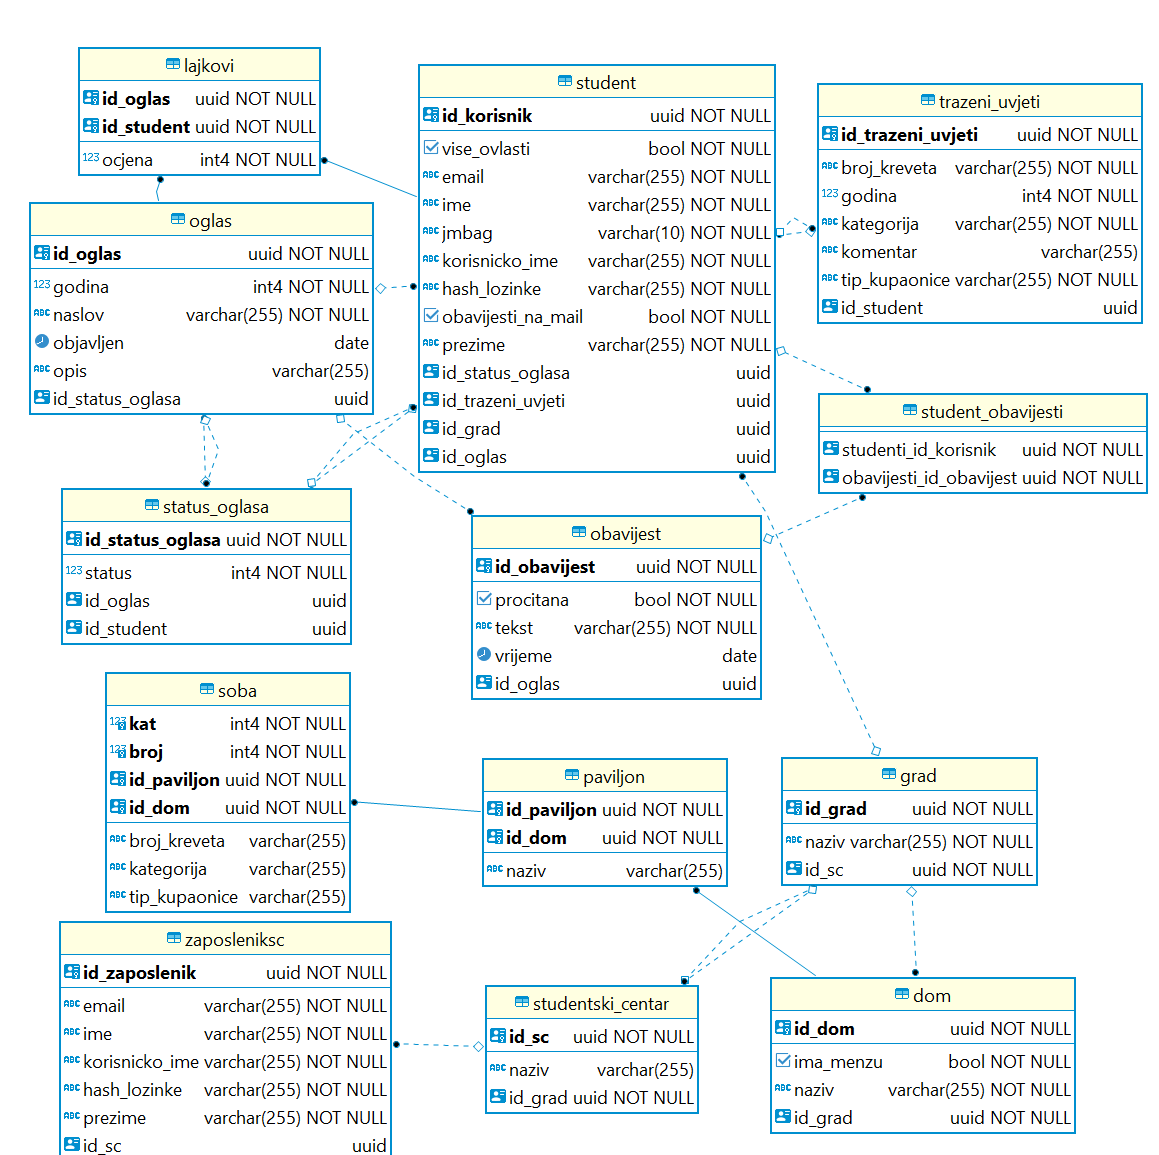
\includegraphics[scale=0.4]{dijagrami/ERdijagram.png} %veličina slike u odnosu na originalnu datoteku i pozicija slike
					\centering
					\caption{ER dijagram baze podataka}
					\label{fig:er}
				\end{figure}
			
			\eject
			
			
		\section{Dijagram razreda}
		
			\textit{Potrebno je priložiti dijagram razreda s pripadajućim opisom. Zbog preglednosti je moguće dijagram razlomiti na više njih, ali moraju biti grupirani prema sličnim razinama apstrakcije i srodnim funkcionalnostima.}\\
			
			\textbf{\textit{dio 1. revizije}}\\
			
			\textit{Prilikom prve predaje projekta, potrebno je priložiti potpuno razrađen dijagram razreda vezan uz \textbf{generičku funkcionalnost} sustava. Ostale funkcionalnosti trebaju biti idejno razrađene u dijagramu sa sljedećim komponentama: nazivi razreda, nazivi metoda i vrste pristupa metodama (npr. javni, zaštićeni), nazivi atributa razreda, veze i odnosi između razreda.}\\
			
			\textbf{\textit{dio 2. revizije}}\\			
			
			\textit{Prilikom druge predaje projekta dijagram razreda i opisi moraju odgovarati stvarnom stanju implementacije}
			
			
			
			\eject
		
		\section{Dijagram stanja}
			
			
			\textbf{\textit{dio 2. revizije}}\\
			
			\textit{Potrebno je priložiti dijagram stanja i opisati ga. Dovoljan je jedan dijagram stanja koji prikazuje \textbf{značajan dio funkcionalnosti} sustava. Na primjer, stanja korisničkog sučelja i tijek korištenja neke ključne funkcionalnosti jesu značajan dio sustava, a registracija i prijava nisu. }
			
			
			\eject 
		
		\section{Dijagram aktivnosti}
			
			\textbf{\textit{dio 2. revizije}}\\
			
			 \textit{Potrebno je priložiti dijagram aktivnosti s pripadajućim opisom. Dijagram aktivnosti treba prikazivati značajan dio sustava.}
			
			\eject
		\section{Dijagram komponenti}
		
			\textbf{\textit{dio 2. revizije}}\\
		
			 \textit{Potrebno je priložiti dijagram komponenti s pripadajućim opisom. Dijagram komponenti treba prikazivati strukturu cijele aplikacije.}
    \chapter*{Popis literature}
		\addcontentsline{toc}{chapter}{Popis literature}
	 	
 		\textbf{\textit{Kontinuirano osvježavanje}}
	
		\textit{Popisati sve reference i literaturu koja je pomogla pri ostvarivanju projekta.}
		
		
		\begin{enumerate}
			
			
			\item  Programsko inženjerstvo, FER ZEMRIS, \url{http://www.fer.hr/predmet/proinz}
			
			\item  I. Sommerville, "Software engineering", 8th ed, Addison Wesley, 2007.
			
			\item  T.C.Lethbridge, R.Langaniere, "Object-Oriented Software Engineering", 2nd ed. McGraw-Hill, 2005.
			
			\item  I. Marsic, Software engineering book``, Department of Electrical and Computer Engineering, Rutgers University, \url{http://www.ece.rutgers.edu/~marsic/books/SE}
			
			\item  The Unified Modeling Language, \url{https://www.uml-diagrams.org/}
			
			\item  Astah Community, \url{http://astah.net/editions/uml-new}
		\end{enumerate}
		
		 
	
	
	\begingroup
	\renewcommand*\listfigurename{Indeks slika i dijagrama}
	%\renewcommand*\listtablename{Indeks tablica}
	%\let\clearpage\relax
	\listoffigures
	%\vspace{10mm}
	%\listoftables
	\endgroup
	\addcontentsline{toc}{chapter}{Indeks slika i dijagrama}
	
	
	
	\eject 
	
	\chapter*{Dodatak: Prikaz aktivnosti grupe}
		\addcontentsline{toc}{chapter}{Dodatak: Prikaz aktivnosti grupe}
		
		\section*{Dnevnik sastajanja}
		
		\begin{packed_enum}
			\item  sastanak
			
			\item[] \begin{packed_item}
				\item Datum: 7. listopada 2020.
				\item Prisustvovali: Mateja Iveta, Dora Horvat, Vedran Hernaus, Lea Brzica, Matija Holik, Denis Đurašinović , Dora Bortas
				\item Teme sastanka:
				\begin{packed_item}
					\item  Upoznavanje članova tima
					\item  Dogovor o tehnologijama. Dogovoreno: Postgres - Spring - React
					\item Dogovor o prijedlogu drugog projektnog zadatka
				\end{packed_item}
			\end{packed_item}
			
			\item  sastanak
			\item[] \begin{packed_item}
				\item Datum: 15. listopada 2020.
				\item Prisustvovali:  Mateja Iveta, Dora Horvat, Vedran Hernaus, Lea Brzica, Matija Holik, Denis Đurašinović , Dora Bortas
				\item Teme sastanka:
				\begin{packed_item}
					\item  Razgovor o funkcionalnim zahtjevima sustava i arhitekturi
					
				\end{packed_item}
			\end{packed_item}
			\item  sastanak
			
			\item[] \begin{packed_item}
				\item Datum: 19. listopada 2020.
				\item Prisustvovali: Mateja Iveta, Dora Horvat, Vedran Hernaus, Lea Brzica, Matija Holik, Denis Đurašinović , Dora Bortas
				\item Teme sastanka:
				\begin{packed_item}
					\item Definiranje organizacije baze podataka
					\item Dogovor o raspodjeli poslova
				\end{packed_item}
			\end{packed_item}
		
			
				\item  sastanak
				
				\item[] \begin{packed_item}
					\item Datum: 22. listopada 2020.
					\item Prisustvovali: Mateja Iveta, Dora Horvat, Vedran Hernaus, Lea Brzica, Matija Holik, Denis Đurašinović , Ivana Cepetić, Luka Martić
					\item Teme sastanka:
					\begin{packed_item}
						\item Razgovor o optimalnoj organizaciji baze podataka
					\end{packed_item}
				\end{packed_item}
				\item  sastanak
			
			\item[] \begin{packed_item}
				\item Datum: 29. listopada 2020.
				\item Prisustvovali: Mateja Iveta, Dora Horvat, Vedran Hernaus, Lea Brzica, Matija Holik, Denis Đurašinović , Dora Bortas
				\item Teme sastanka:
				\begin{packed_item}
					\item Podjela uloga za kreiranje baze, izradu kontrolera, servisa i repozitorija, dokumentacije i logina i registgracije
				\end{packed_item}
			\end{packed_item}
		 \item sastanak
		\item[] \begin{packed_item}
			\item Datum: 4. studenoga 2020.
			\item Prisustvovali:  Dora Horvat, Dora Bortas, Ivana Cepetić, Luka Martić
			\item Teme sastanka:
			\begin{packed_item}
				\item Razgovor o trenutnom napretku dokumentacije
				
			\end{packed_item}
		\end{packed_item}
	\item sastanak
		\item[] \begin{packed_item}
			\item Datum: 6. studenoga 2020.
			\item Prisustvovali: Mateja Iveta, Dora Horvat, Vedran Hernaus, Lea Brzica, Matija Holik, Denis Đurašinović , Dora Bortas
			\item Teme sastanka:
			\begin{packed_item}
				\item Diskusija o trenutnom napretku projekta
				\item Podjela poslova koji se moraju obaviti do prve predaje projekta
			\end{packed_item}
		\end{packed_item}
	
		\item sastanak
		\item[] \begin{packed_item}
			\item Datum: 10. studenoga 2020.
			\item: Prisustvovali: Mateja Iveta, Dora Horvat, Vedran Hernaus, Lea Brzica, Matija Holik, Denis Đurašinović , Dora Bortas
			\item Teme sastanka:
			\begin{packed_item}
				\item Dogovor o načinu kriptiranja i hashiranju lozinki
			\end{packed_item}
		\end{packed_item}
	
			\item sastanak
		\item[] \begin{packed_item}
			\item Datum: 11. studenoga 2020.
			\item: Prisustvovali: Mateja Iveta, Dora Horvat, Vedran Hernaus, Lea Brzica, Matija Holik, Denis Đurašinović , Dora Bortas
			\item Teme sastanka:
			\begin{packed_item}
				\item Pregled trenutnog stanja projekta
				\item Priprema za prvo kolokviranje
				
			\end{packed_item}
		\end{packed_item}
	
			\item sastanak
			\item[] \begin{packed_item}
				\item Datum: 12. studenoga 2020.
				\item Prisustvovali: Mateja Iveta, Dora Horvat, Vedran Hernaus, Lea Brzica, Matija Holik, Denis Đurašinović , Dora Bortas, Ivana Cepetić, Luka Martić, Hrvoje Šimić
				\item Teme sastanka:
				\begin{packed_item}
					\item Pregled generičkih funkcionalnosti aplikacije prije prve predaje
				\end{packed_item}
			\end{packed_item}
		
			\item sastanak
			\item[] \begin{packed_item}
				\item Datum: 3. prosinca 2020.
				\item Prisustvovali: Mateja Iveta, Dora Horvat, Vedran Hernaus, Lea Brzica, Matija Holik, Denis Đurašinović , Dora Bortas, Ivana Cepetić, Hrvoje Šimić
				\item Teme sastanka:
				\begin{packed_item}
					\item Kolokviranje prvog ciklusa projekta
				\end{packed_item}
			\end{packed_item}
		
			\item sastanak
			\item[] \begin{packed_item}
				\item Datum: 10. prosinca 2020.
				\item Prisustvovali: Mateja Iveta, Dora Horvat, Vedran Hernaus, Lea Brzica, Matija Holik, Denis Đurašinović , Dora Bortas
				\item Teme sastanka:
				\begin{packed_item}
					\item Podjela poslovna nakon kolokviranja
				\end{packed_item}
			\end{packed_item}
		
			\item sastanak
			\item[] \begin{packed_item}
				\item Datum: 29. prosinca 2020.
				\item Prisustvovali: Mateja Iveta, Dora Horvat, Vedran Hernaus, Lea Brzica, Matija Holik, Denis Đurašinović , Dora Bortas
				\item Teme sastanka:
				\begin{packed_item}
					\item Provjera napretka projekta
					\item Ponovna podjela zadataka
				\end{packed_item}
			\end{packed_item}
		
			\item sastanak
			\item[] \begin{packed_item}
				\item Datum: 31. prosinca 2020.
				\item Prisustvovali: Mateja Iveta, Dora Horvat, Vedran Hernaus, Lea Brzica, Matija Holik, Denis Đurašinović , Dora Bortas
				\item Teme sastanka:
				\begin{packed_item}
					\item Provjera napretka projekta
				\end{packed_item}
			\end{packed_item}
		
			\item sastanak
			\item[] \begin{packed_item}
				\item Datum: 2. siječnja 2021.
				\item Prisustvovali: Mateja Iveta, Dora Horvat, Vedran Hernaus, Lea Brzica, Matija Holik, Denis Đurašinović , Dora Bortas
				\item Teme sastanka:
				\begin{packed_item}
					\item Dogovor o implementaciji lajkova
				\end{packed_item}
			\end{packed_item}
		
			\item sastanak
			\item[] \begin{packed_item}
				\item Datum: 3. siječnja 2021.
				\item Prisustvovali: Mateja Iveta, Dora Horvat, Vedran Hernaus, Lea Brzica, Matija Holik, Denis Đurašinović , Dora Bortas
				\item Teme sastanka:
				\begin{packed_item}
					\item Dogovor o algoritmu uparivanja oglasa
				\end{packed_item}
			\end{packed_item}
		
			\item sastanak
			\item[] \begin{packed_item}
				\item Datum: 4. siječnja 2021.
				\item Prisustvovali: Mateja Iveta, Dora Horvat, Vedran Hernaus, Lea Brzica, Matija Holik, Denis Đurašinović , Dora Bortas
				\item Teme sastanka:
				\begin{packed_item}
					\item Provjera napretka
					\item Dogovor o nastavku rada na aplikaciji
				\end{packed_item}
			\end{packed_item}
		
			\item sastanak
			\item[] \begin{packed_item}
				\item Datum: 7. siječnja 2021.
				\item Prisustvovali: Mateja Iveta, Dora Horvat, Vedran Hernaus, Lea Brzica, Matija Holik, Denis Đurašinović , Dora Bortas, Ivana Cepetić
				\item Teme sastanka:
				\begin{packed_item}
					\item Prezentacija alfa verzije projekta
				\end{packed_item}
			\end{packed_item}
			
			%
			
		\end{packed_enum}
		
		\eject
		\section*{Tablica aktivnosti}
		
						
			
			\begin{longtabu} to \textwidth {|X[7, l]|X[1, c]|X[1, c]|X[1, c]|X[1, c]|X[1, c]|X[1, c]|X[1, c]|}
								
				\cline{2-8} \multicolumn{1}{c|}{\textbf{}} &     \multicolumn{1}{c|}{\rotatebox{90}{\textbf{ Mateja Iveta }}} & \multicolumn{1}{c|}{\rotatebox{90}{\textbf{Dora Bortas }}} &	\multicolumn{1}{c|}{\rotatebox{90}{\textbf{Dora Horvat }}} &	\multicolumn{1}{c|}{\rotatebox{90}{\textbf{Lea Brzica }}} &
				\multicolumn{1}{c|}{\rotatebox{90}{\textbf{Vedran Hernaus }}} &
				\multicolumn{1}{c|}{\rotatebox{90}{\textbf{Matija Holik }}} &	\multicolumn{1}{c|}{\rotatebox{90}{\textbf{Denis Đurašinović }}} \\ \hline 
				\endfirsthead
				
			
				\cline{2-8} \multicolumn{1}{c|}{\textbf{}} &     \multicolumn{1}{c|}{\rotatebox{90}{\textbf{Mateja Iveta}}} & \multicolumn{1}{c|}{\rotatebox{90}{\textbf{Dora Bortas }}} &	\multicolumn{1}{c|}{\rotatebox{90}{\textbf{Dora Horvat }}} &
				\multicolumn{1}{c|}{\rotatebox{90}{\textbf{Lea Brzica }}} &	\multicolumn{1}{c|}{\rotatebox{90}{\textbf{Vedran Hernaus }}} &
				\multicolumn{1}{c|}{\rotatebox{90}{\textbf{Matija Holik }}} &	\multicolumn{1}{c|}{\rotatebox{90}{\textbf{Denis Đurašinović }}} \\ \hline 
				\endhead
				
				
				\endfoot
							
				 
				\endlastfoot
				
				Upravljanje projektom 		& 5 &  &  &  &  &  & \\ \hline
				Opis projektnog zadatka 	&  &  & 6 &  &  &  & \\ \hline
				
				Funkcionalni zahtjevi       &  & 3 &  &  &  &  &  \\ \hline
				Opis pojedinih obrazaca 	&  & 5 &  &  &  &  &  \\ \hline
				Dijagram obrazaca 			&  & 5 &  &  &  &  &  \\ \hline
				Sekvencijski dijagrami 		&  & 3 &  &  &  &  &  \\ \hline
				Opis ostalih zahtjeva 		&  & 1 &  &  &  &  &  \\ \hline

				Arhitektura i dizajn sustava&  & 1 &  &  &  &  &  \\ \hline
				Baza podataka				&  &  & 15 &  &  &  &   \\ \hline
				Dijagram razreda 			&  & 5 & 5 &  &  &  &   \\ \hline
				Dijagram stanja				&  &  & 8 &  &  &  &  \\ \hline
				Dijagram aktivnosti 		&  &  & 8 &  &  &  &  \\ \hline
				Dijagram komponenti			&  &  & 8 &  &  &  &  \\ \hline
				Korištene tehnologije i alati 		& 5 &  &  &  &  &  &  \\ \hline
				Ispitivanje programskog rješenja 	&  & 10 &  &  &  &  &  \\ \hline
				Dijagram razmještaja			&  &  & 5 &  &  &  &  \\ \hline
				Upute za puštanje u pogon 		&  &  & 6 &  &  &  &  \\ \hline 
				Dnevnik sastajanja 			&  &  & 1 &  &  &  &  \\ \hline
				Zaključak i budući rad 		&  &  & 3 &  &  &  &  \\  \hline
				Popis literature 			&  &  &  &  &  &  &  \\  \hline
				&  &  &  &  &  &  &  \\ \hline \hline
				Izrada frontenda 		 	& 50 & 20 &  & 50 & 50 & 2 &  \\ \hline
				Izrada backenda 		 	& 50 & 10 &  & 10 & 20 & 50 & 30 \\ \hline 
				Sigurnost					& 5 &  &  &  &  & 30 & \\ \hline 
				Spajanje na bazu 		 	& 5  &  &  &  &  & 5 & 5 \\ \hline 
				Modeliranje baze 			& 5 & 2 &  &  &  & 10 & 30 \\ \hline
				Puštanje u pogon		 	& 15  &  &  &  &  &  &  \\  \hline
				 						
				
				
			\end{longtabu}
					
					
		\eject
		
		\section*{Dijagrami pregleda promjena}
		
		\begin{figure}[H]
			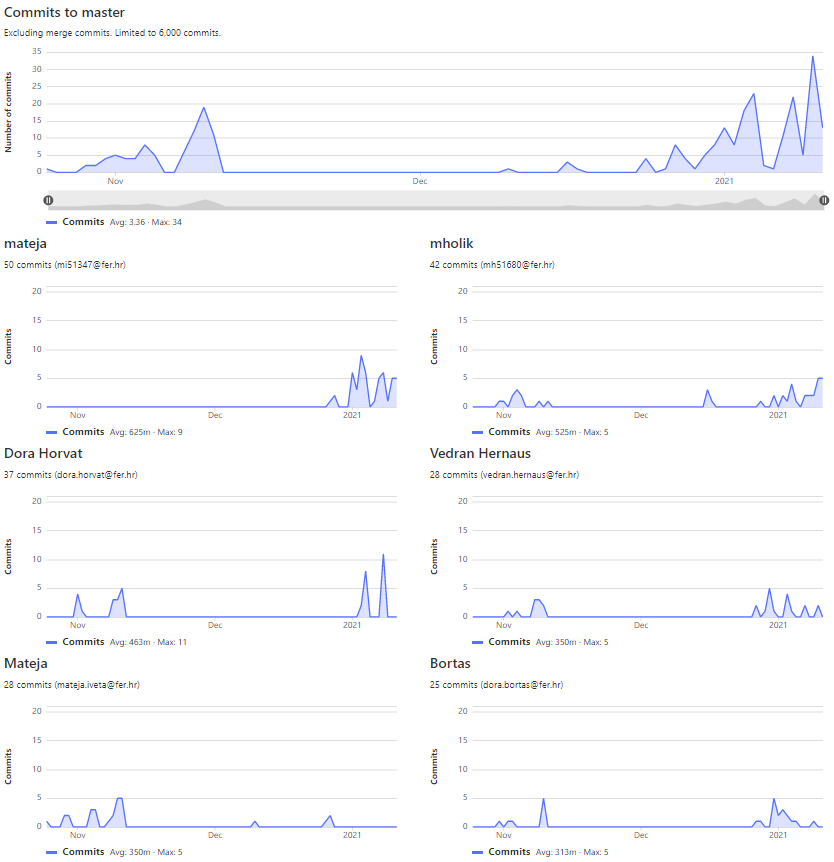
\includegraphics[scale=0.7]{slike/gitlab1.png} %veličina slike u odnosu na originalnu datoteku i pozicija slike
			\centering
			\caption{Dijagrami aktivnosti na master grani}
			\label{fig:aktivnost1}
		\end{figure}
	
		\begin{figure}[H]
			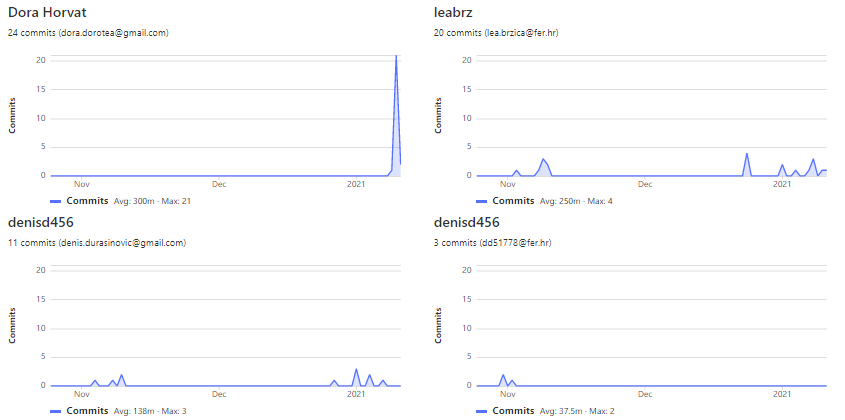
\includegraphics[scale=0.7]{slike/gitlab2.png} %veličina slike u odnosu na originalnu datoteku i pozicija slike
			\centering
			\caption{Dijagrami aktivnosti na master grani}
			\label{fig:aktivnost2}
		\end{figure}
		

	
	
\end{document} %naredbe i tekst nakon ove naredbe ne ulaze u izgrađen dokument 


